%
% problemstellung.tex -- Beispiel-File für die Beschreibung des Problems
%
% (c) 2020 Prof Dr Andreas Müller, Hochschule Rapperswil
%
\section{Beispiele
\label{logistic:section:folgerungen}}
\rhead{Beispiele}

In Kapitel \ref{logistic:section:problemstellung} 
haben wir bereits gesehen, 
dass das Bifurkationsdiagramm der logistischen Gleichung
ein Fraktal ist. 
Eines der bekanntesten Fraktale ist die Mandelbrotmenge,
wessen Gleichung der logistischen Gleichung sehr ähnlich ist. 
Die Gleichung der Mandelbrotmenge lautet
\begin{equation}
    z_{n+1} = z_n^2 + c
    \label{eq:mandelbrot}
\end{equation}
wobei $z_n$ und $c$ komplexe Zahlen sind und 
der Einfachkeit halber $z_0 = 0$ gesetzt werden kann.
Zum Vergleich, die logistische Gleichung hat ausmultipliziert
die Form $x_{n+1} = -\lambda x_n^2 +\lambda x_n$. 
Wie bei der logistischen Gleichung gibt es auch
bei der Gleichung der Mandelbrotmenge wieder bestimmte
Werte von $c$, bei der $z_n$ entweder 
divergiert, 
konvergiert, 
oszilliert 
oder in chaotisches Verhalten ausbricht. 
Jeder Wert von $c$ für den $z_n$ nicht 
divergiert ist Teil der Mandelbrotmenge. 
Nun können wir, ähnlich wie schon beim 
Bifurkationendiagramm der logistischen Gleichung, auf der
komplexen Ebene für jeden Wert von $c$ das Verhalten
der Gleichung der Mandelbrotmenge darstellen. 
Wenn $z_n$ divergiert dann wird der Punkt weiss
eingefärbt, sonst schwarz. 
Damit sehen wir auf Abbildung \ref{fig:mandel_2d}
die Mandelbrotmenge. 
\begin{figure}
    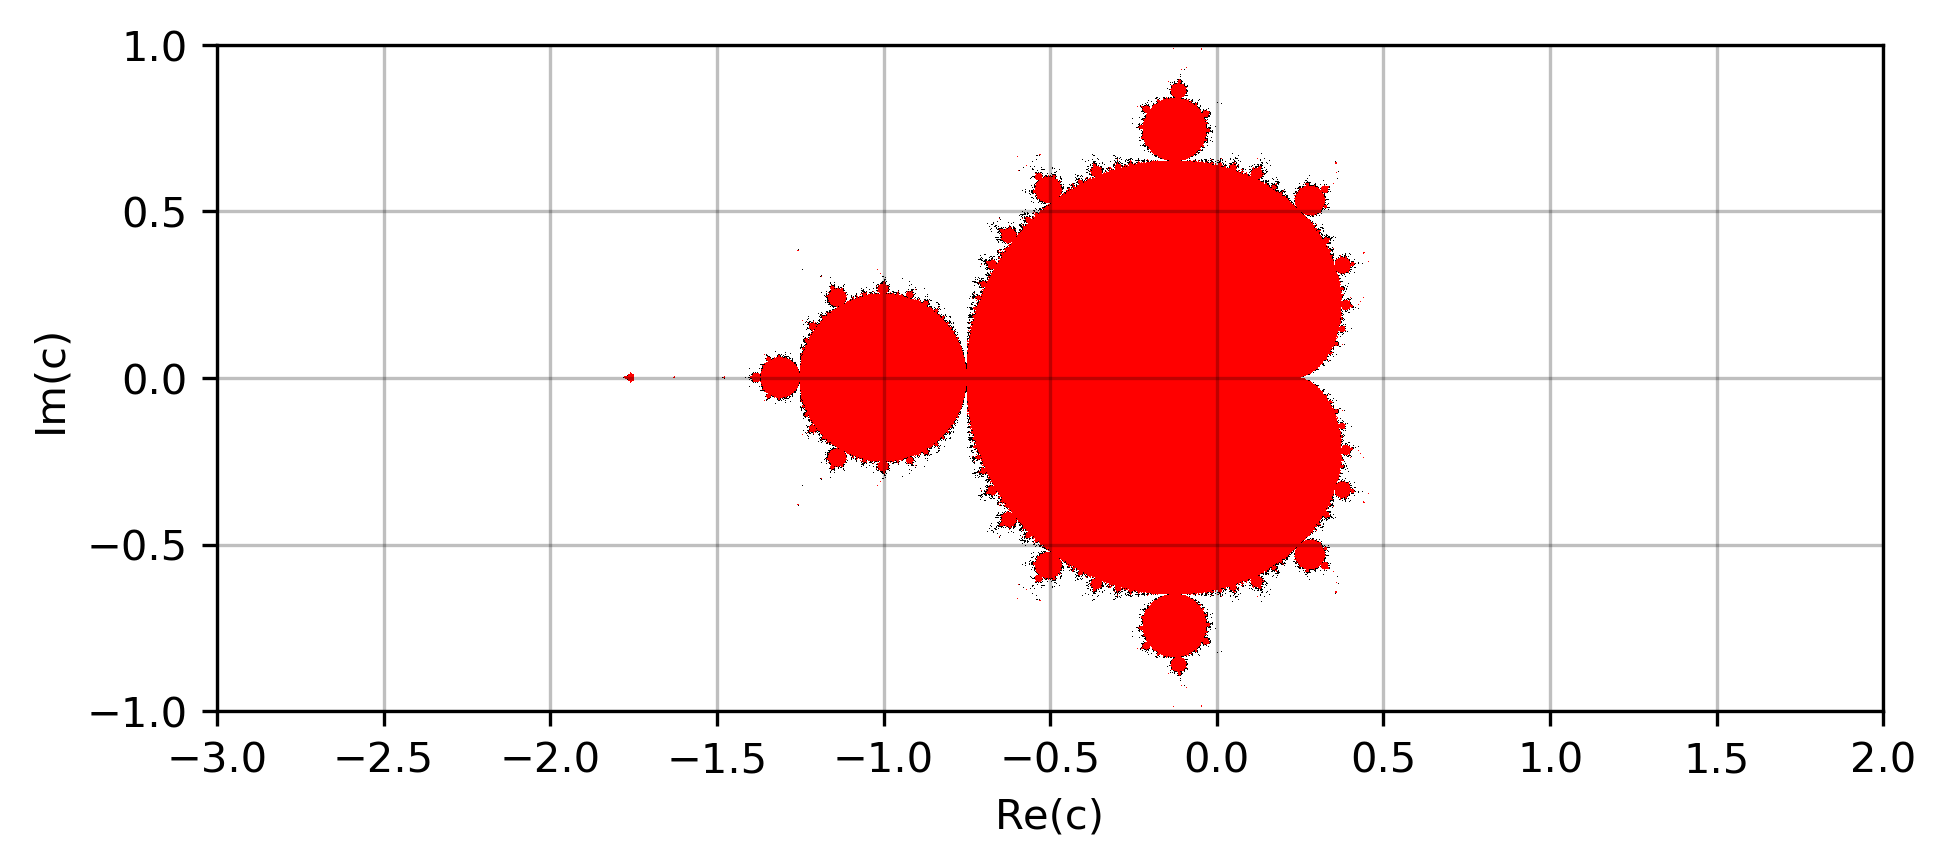
\includegraphics[width=\linewidth]{papers/logistic/figures/mandel.png}
    \caption{Mandelbrotmenge}
    \label{fig:mandel_2d}
\end{figure}
Auf dieser zweidimensionalen Darstellung 
ist jedoch nicht zu sehen, welche
Werte $z_n$ annimmt, nur ob es konvergiert oder divergiert.
Darum nehmen wir jetzt die dritte Dimension zur Hilfe um,
wie schon beim Bifurkationendiagramm der logistischen Gleichung,
auf der vertikalen Achse darzustellen, 
auf welchem Wert sich $z_n$ schlussendlich einpendelt.
Oder eben auch nicht, wenn es oszilliert oder sogar
chaotisch wird. 
Das Ergebnis davon ist auf Abbildung 
\ref{fig:mandel_3d}
zu sehen. 
Auf der reellen Achse ist deutlich ein Gebilde zu sehen,
welches dem Bifurkationendiagramm der logistischen
Gleichung sehr ähnlich sieht. 
Ebenfalls zu sehen ist, dass die kreisförmigen
``Platformen'' sich regelmässig verdoppeln, weil
$z_n$ zwischen immer mehr Werten hin und her oszilliert. 
\begin{figure}
    
\includegraphics[width=\linewidth]{papers/logistic/figures/mandel_3d.png}
    \caption{Bifurkationsdiagramm der Mandelbrotmenge}
    \label{fig:mandel_3d}
\end{figure}

Damit kommen wir auch schon zum nächsten Punkt. 
Dieses ganze Verhalten mit den Periodenverdoppelungen und
immer wieder kurzen oszillierenden Fenstern im Chaos
ist keineswegs eine Eigenschaft, 
die nur die logistische Gleichung besitzt.
Man findet dieses Verhalten auch beim Iterieren 
von vielen anderen nichtlinearen Funktionen. 
TODO beispiele ...

TODO dripping faucet